%%%%%%%%%%%%%%%%%%%%%%%%%%%%%%%%%%%%%%%%%
% FRI Data Science_report LaTeX Template
% Version 1.0 (28/1/2020)
% 
% Jure Demšar (jure.demsar@fri.uni-lj.si)
%
% Based on MicromouseSymp article template by:
% Mathias Legrand (legrand.mathias@gmail.com) 
% With extensive modifications by:
% Antonio Valente (antonio.luis.valente@gmail.com)
%
% License:
% CC BY-NC-SA 3.0 (http://creativecommons.org/licenses/by-nc-sa/3.0/)
%
%%%%%%%%%%%%%%%%%%%%%%%%%%%%%%%%%%%%%%%%%


%----------------------------------------------------------------------------------------
%	PACKAGES AND OTHER DOCUMENT CONFIGURATIONS
%----------------------------------------------------------------------------------------
\documentclass[fleqn,moreauthors,10pt]{ds_report}
\usepackage[english]{babel}

\usepackage{placeins}
\usepackage{comment}
\usepackage{adjustbox}

% array packages
\usepackage{array}
\usepackage{tabularx} 
\usepackage{changepage}
\usepackage{placeins}
\usepackage{makecell}
\usepackage{multirow} 
\usepackage{float}

\graphicspath{{fig/}}




%----------------------------------------------------------------------------------------
%	ARTICLE INFORMATION
%----------------------------------------------------------------------------------------

% Header
\JournalInfo{FRI Natural language processing course 2026}

% Interim or final report
\Archive{Project report} 
%\Archive{Final report} 

% Article title
\PaperTitle{Conversational Recommender System for Vehicles} 

% Authors (student competitors) and their info
\Authors{Primož Gabrovec, Rožle Sterle and Zala Urh}

% Advisors
\affiliation{\textit{Advisors: Aleš Žagar}}

% Keywords
\Keywords{Conversational Recommender System, RAG, FAISS, Car recommendation, LLM}
\newcommand{\keywordname}{Keywords}


%----------------------------------------------------------------------------------------
%	ABSTRACT
%----------------------------------------------------------------------------------------

\Abstract{
In this report, we design a Conversational Recommender System for vehicle selection. 
The system helps users express their preferences in natural language and translates them 
structured technical terms. We propose a dual data strategy that combines 
two data retrieval approaches. The first is constraint-based filtering over a structured 
SQL-like database of vehicle attributes. The second is FAISS-based similarity search 
over vector embeddings generated from vehicle brochures.
We evaluate the proposed system against multiple variants. LLM such as Qwen and LLama without any 
data retrieval represents the baseline. More advanced comparison represent 
a non-conversational version of the proposed recommender system.
In all cases the proposed recommender system outperformed the others.
}
%\textbf{TODO! Dodaj dejanske rezultate al neki}

%----------------------------------------------------------------------------------------

\begin{document}

% Makes all text pages the same height
\flushbottom 

% Print the title and abstract box
\maketitle 

% Removes page numbering from the first page
\thispagestyle{empty} 

%----------------------------------------------------------------------------------------
%	ARTICLE CONTENTS
%----------------------------------------------------------------------------------------

\section*{Introduction}
In the past years, choosing a suitable vehicle has become very challenging due to a wide range of options. Customers can choose between many models with different fuel types, engine characteristics, size, and other specifics. 

Most existing systems that assist users in selecting vehicles are based on predefined filters, such as price range, brand, transmission types, and others. While this approach is effective for experienced users, it might not be that suitable for those who cannot easily translate their needs into technical details.

As an improvement to such systems, Conversational Recommender Systems (CRS) have been introduced. A CRS is an interactive system that allows users to express their preferences through dialogue, while the system can ask follow-up questions to refine these preferences and provide the best recommendation(s). 

In this paper, we propose a hybrid CRS for vehicle selection using that combines large 
language models (LLMs), structured constraint extraction, and retrieval-augmented generation (RAG). 
The system engages the user in a conversation with an LLM that helps them express and refine their vehicle preferences.
The final product is a system that simplifies making a 
decision for non-expert users, and also improves customer experience in vehicle selling companies.



\section*{Related work}
Several studies have explored recommender systems, however the vehicle domain remains limited. We categorized existing work into recommendation systems for vehicles and conversational recommender systems for various products.

In the context of vehicle recommendation, Beddouda et al. \cite{beddoudavehicle} proposed a system using BERT4Rec, which predicts which cars a user might be interested in based on past interactions (without any user communication). Singh et al. \cite{singh2022car} introduced a one-turn dialogue system that uses LDA model to analyse user reviews, where users describe their car preferences and the system returns top few recommendations.

For general CRS, several multi-turn dialogue systems have been proposed, especially in the travel domain. Liao et al. \cite{liao2019deepconversationalrecommendertravel} proposed a deep recommender system using seq2seq with a neural latent topic component. Baizal et al. \cite{baizal2021tourism} introduced an ontology-based system, and Carrillo et al. \cite{carrillo2023smarttur+} introduced a system that uses Chatbot to collect user preferences and generates similarity-based recommendations using SBERT embeddings.

In addition to the travel domain, CRS have been implemented in several other domains. Sun et al. \cite{sun2018conversational} developed a reinforcement learning based CRS for restaurant recommendation using Yelp review data. Zhu et al. \cite{zhu2025collaborative} proposed a movie recommendation CRS using retrieval-augmented generation (RAG) approach in combination with a large language model.


%------------------------------------------------

\section*{Methods}

The proposed system is designed as a Conversational Recommender System (CRS) 
that integrates large language models (LLMs), 
structured data processing, and retrieval-augmented generation (RAG) to provide personalized 
vehicle recommendations through natural 
language interaction. The overall pipeline is described below as well as shown
on the figure \ref{CRS diagram}.


\subsubsection*{Data Preprocessing} \label{data processing}

The first dataset was extracted from the CarAPI website \cite{carapi}. 
It provides vehicle data in JSON format, such as price, fuel consumption, 
engine specifications... Data was then processed and stored into 
structured SQLite database (on Figure \ref{CRS diagram} marked as Structured database). 

The second dataset consists of vehicle brochures in PDF format
extracted from the Auto-Brochures website \cite{autobrochuers}. 
The dataset includes 
multiple car brands available on the US market, of which 26 were selected 
for this work. We used a Qwen embedding model to generate vector 
represenations of the dataset content. These embeddings were then 
indexed using FAISS (Facebook AI similarity search) \cite{faiss}
to enable efficient similarity search (Dataset
is marked on Figure \ref{CRS diagram} as FAISS Vector Database).


\subsubsection*{Conversational Recommender System - CRS}

The system begins with user describing in natural language their preferences and requirements 
they look for in a new car. That input is then parsed by the LLM (on figure 
\ref{CRS diagram} marked as LLM Parser). 

Parsing is implemented by first extracting relevant attributes from the user's query using the embeddings of the description of the attributes. When we defined a schema for the structured database, we also crafted metadata for each attribute in a form of a short description. This description also includes synonyms, related terms, user intentions and example queries. Then we embed those descriptions using an embedding model, which was selected with benchmarking of different models, with a specialised instructions for the task. When the user query is received, we embed it using the same embedding model and then calculate similarity between the query embedding and the attribute description embeddings. The attributes with the highest similarity are selected as relevant to the user's query.

For each relevant attribute, the LLM is then prompted to extract the corresponding value and constraint, which proved to be more effective than directly prompting the LLM to extract every attribute at once. 

Table \ref{tab:parsed query example} shows an example of the extracted structured information from a user query. The LLM is able to identify that the user is looking for an SUV with electric engine, but it cannot determine the exact value of the fuel consumption constraint, which is then marked as None.

\begin{table}[H]
\resizebox{1.0 \linewidth}{!}
{\begin{tabular}{| c c c |}

\hline
Name & Value & \makecell{Constraint \\ (min, max, equal...)}  \\ 
\hline
body\_type  & SUV & equal  \\
\hline
engine\_type  & electric & equal  \\
\hline
combined\_l\_per\_100km  & None & None  \\
\hline

\end{tabular}}
\caption{
    Example of parsed text for the following user's query: 
    "I'm looking for a spacious SUV with low consumption, preferably electric."
}
\label{tab:parsed query example}
\end{table}
\FloatBarrier

That is why a single user query is usually not enough to generate a good recommendation. User also might not express all their preferences in a single query, leading to a very large choice of cars. 

\vspace{3pt}
\noindent
To address these issues, we improved the system with creating a conversational LLM
(marked on Figure \ref{CRS diagram} with the same name). This model 
interacts with the user to complete missing constraints and suggest additional 
attributes that could be in interest to the user.

Then the system employs a dual data strategy using data-bases described
in the previous section.
First, we fetch relevant cars from the database using constraint-based filtering,
which yields the first candidate set. Next we embed the user's query, along with the system's conversation history, and use it for semantic search in the FAISS vector database. Which contains embedded chunks from the vehicle brochures. This allows the system to retrieve cars that are semantically similar to the user's preferences, even if they do not exactly match the structured constraints. While we can extract information such as number of seats, or fuel type from the structured database, other information such as a car's feel, design or equipment is not easily captured in structured form, but can be retrieved from the brochures using the semantic search.

The system then combines both retrieved sets of car candidates and filters them again to ensure that candidates from the FAISS search also meet the user's constraints. The contex of the retrieved chunks is then correctly formatted and provided to the LLM as part of the final recommendation prompt. So the LLM can summarize the retrieved information and generate a final recommendation response. The LLM also comments on the key differences between the suggested cars, which can help users make an informed decision. 


\begin{figure}[!htbp]
    \centering
    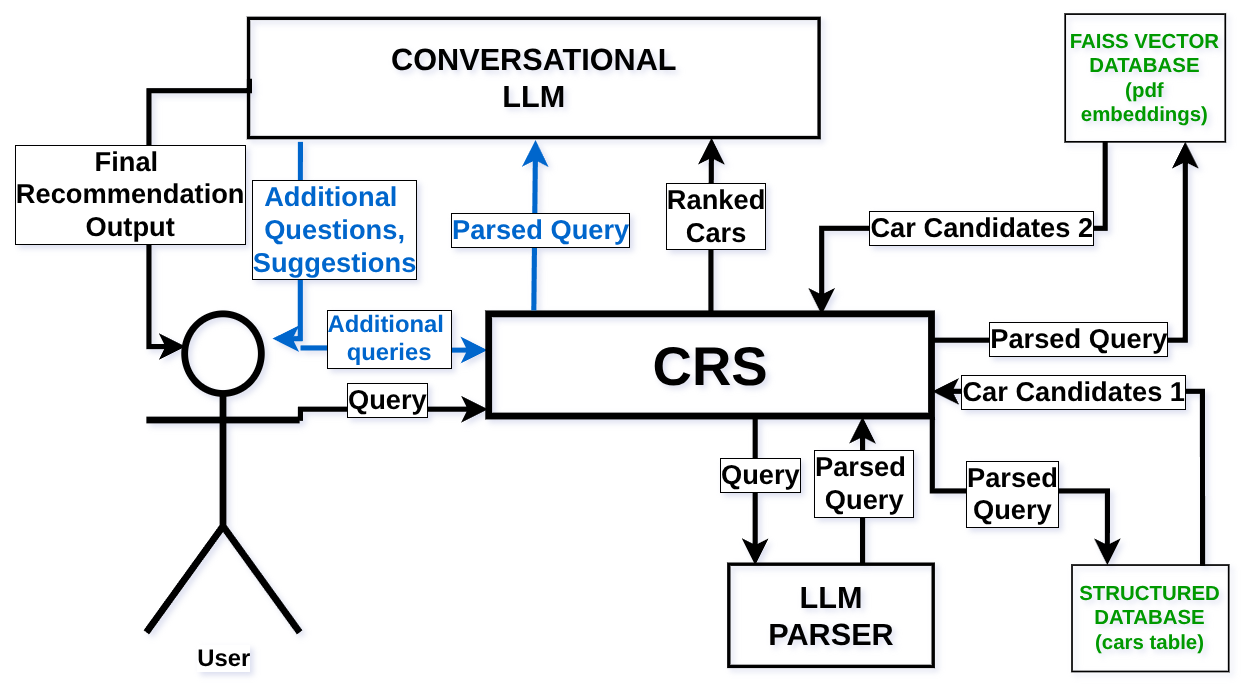
\includegraphics[width=\columnwidth]{fig/crs_system.png} 
    \caption{
        CRS Architecture. Blue arrows represent conversation interaction loop between the 
        user and the LLM, green components represent databases that the system uses.
    }
    \label{CRS diagram}
\end{figure}
\FloatBarrier




\section*{Evaluation methods and Results}

We designed two types of tests: the ones that evaluate the embedded model, 
and the ones that evaluate the final system. 

\subsubsection*{Attribute embeddings evaluation}

We designed a benchmark to evaluate the performance of different embedding models for 
the task of identifying relevant attributes from user queries. We created a dataset of 
40 user queries, each manually annotated with the relevant attributes. We then tested 
several embedding models, from Qwen, BAAI-bge, nomic-ai, GTE, Google's gemma and jinaai. 
To rank the models we measured Spearman's correlation to measure how well the model's 
ranking of attributes agrees with the ground truth (Agreement). We also measured the separation with 
Cohen's \(d\), since we want a large distance between the relevant and irrelevant attributes,
and finally we also measured the F1 score, which was also optimized with different thresholds.
 
\vspace{5pt}
\noindent
Results of evaluations of the embedded models with their optimal thresholds are shown in the
Table \ref{tab:benchmark results}. In  the end, Qwen3-Embedding-0.6B model 
was chosen since it was the best trade-off between its performance and speed.
% \texttt{\textbf{Qwen3-Embedding-0.6B}}
\begin{table}[H]
\resizebox{1.0 \linewidth}{!}
{\begin{tabular}{| c | c || c c c c |}

\hline
Model & Threshold &  Agreement & Separation & F1  & \makecell{Final \\ score} \\ 
\hline
\makecell{Qwen/Qwen3 \\ Embedding-4B}  &  0.57 &  0.40 & 1.65 & 0.57 & 0.87 \\
\hline
\makecell{jinaai/jina-embeddings \\ v5-text-small}  &  0.33 &  0.39 & 1.61 & 0.52 & 0.84 \\
\hline
\makecell{Qwen/Qwen3 \\ Embedding-0.6B}  &  0.49 &  0.40 & 1.58 & 0.53 & 0.84 \\
\hline
\makecell{google/embeddinggemma \\ 300m}  &  0.29 &  0.39 & 1.59 & 0.51 & 0.83 \\
\hline
\makecell{jinaai/jina-embeddings \\ v5-text-nano}   &  0.33 & 0.38 & 1.55 & 0.54 & 0.83 \\
\hline
 ... & ... & ... & ... & ... &  \\
\hline


\end{tabular}}
\caption{
    Results of performances of different embedding models
}
\label{tab:benchmark results}
\end{table}
\FloatBarrier


\subsubsection*{Model evaluation}


%\textbf{TODO: add LLM's names} 

Evaluating language models is challenging because their outputs are not 
fully deterministic, especially when they are in conversation mode. We 
designed three different tests to evaluate the system and the models.

First, we evaluate whether the system performs better than a baseline. 
We manually created a set of user queries and manually parsed them into 
constraints (similar to Table \ref{tab:parsed query example}). 
We then ran our system in non-conversational mode, 
which directly returns a set of recommended cars. This result is compared 
to the set of cars obtained from the structured database using the manually 
verified constraints. From this comparison, we compute standard metrics 
such as number of correctly retrieved cars, missed cars, precision, recall, 
and F1 score. We also run the same evaluation for a baseline LLM without 
any system support.

The second evaluation tests the conversational setup. This evaluation 
is not fully automated. We use the same queries as before, but divide them 
into few parts. We simulate 
multi-turn interaction by providing additional part after each LLM question. 
After the conversation ends, we store the final set of recommended cars and 
compare it to the expected set obtained from the structured database using 
the manually parsed query. We also compare that to two baselines

\vspace{5pt}
\noindent
Results of the two tests:

\begin{table}[H]
\resizebox{1.0 \linewidth}{!}
{\begin{tabular}{| c | c c c |}

\hline
%Model & \makecell{number of \\ correctly retrieved \\ cars} & \makecell{number of \\ missed \\ cars} & precision  & recall & F1 \\ 
Model & \makecell{number of \\ correctly retrieved \\ cars} & \makecell{number of \\ missed \\ cars} & recall \\ \hline
\makecell{baseline LLM \\ Qwen}  &  2  & 15 & 0.12 \\
\hline
\makecell{CRS \\ non-conversational \\ Mistral}  &  0  & 17 & 0.00 \\
\hline
\makecell{CRS \\ non-conversational \\ Qwen}  &  14 & 3  & 0.82 \\
\hline
\makecell{CRS \\ conversational \\ Qwen}  &  14 & 3  & 0.82 \\
\hline

\end{tabular}}
\caption{
    Results of the first and second evaluation tests
}
\label{tab:CRS results}
\end{table}
\FloatBarrier



The third evaluation tests whether the RAG component is working correctly.
After each recommendation, we manually check whether the returned cars 
satisfy the user's stated preferences.


\begin{table}[H]
\resizebox{1.0 \linewidth}{!}
{\begin{tabular}{| c | c c c  |}

\hline
Model & \makecell{number of user's \\ preferences} & \makecell{number of satisfied \\ user's preferences} & precentage \\ 
\hline
baseline LLM  &  5 &  3 & 0.6  \\
\hline
\makecell{CRS \\ non-conversational}  &  5 &  5 & 1.0  \\
\hline
\makecell{CRS \\ conversational}   &  5 &  5 & 1.0  \\
\hline

\end{tabular}}
\caption{
    Results of the third evaluation tests
}
\label{tab:CRS results constraints}
\end{table}
\FloatBarrier



%------------------------------------------------




\subsubsection*{Example conversation}

We also present one of the example conversation flow 
between user and our system:

\vspace{3pt}
\noindent
\underline{User:} I am looking for an affordable family SUV with 7 seats.

\noindent
\underline{Assistant:} To help narrow down your options, could you please specify if you prefer a particular make or model? Additionally, do you have any requirements regarding the fuel type or the seating arrangement like second-row captain's chairs versus a bench seat?

\vspace{3pt}
\noindent
\underline{User:} I do not have a brand or model preference, but I would like to have a diesel engine.

\noindent
\underline{Assistant:} 
Given your preference for a diesel engine and need for a 7-seater SUV, I recommend focusing 
on the Audi Q7, Chevrolet Suburban, and Chevrolet Tahoe. These models balance affordability:

\begin{enumerate}
    \item **Audi Q7**: Offers robust performance and luxurious interiors suitable for a family. However, note that finding a diesel variant might be limited due to market availability, typically preferring gasoline engines. 
    \item **Chevrolet Suburban**: Provides ample space and reliable diesel option, ideal for large families needing extra room. It's known for durability and comfort, making long journeys easier.
    \item **Chevrolet Tahoe**: Another strong contender offering a comfortable ride and sufficient seating capacity. Like the Suburban, it has a diesel version which ensures good fuel efficiency and lower running costs over time.
\end{enumerate}

\noindent
While the Mercedes-Benz models offer premium features, they tend to be more expensive and less common 
in diesel versions. The Land Rover Discovery is also a great choice, though it primarily uses petrol 
engines and is priced higher than the others mentioned here.

\noindent
For your specific needs, the **Suburban** and **Tahoe** stand out due to their reliability, spaciousness, 
and availability of diesel engines, balancing practicality and cost-effectiveness well.

\noindent
Top Recommendations:

\begin{enumerate}[itemsep=0pt, topsep=0pt]
    \item Audi Q7
    \item Land Rover Discovery
    \item Mercedes-Benz GL-Class
    \item Mercedes-Benz GLS-Class
    \item Chevrolet Suburban
    \item Chevrolet Tahoe
\end{enumerate}

%------------------------------------------------

\section*{Discussion}

As seen in the table \ref{tab:CRS results}, the proposed recommender system 
outperforms the baseline LLM across all evaluation metrics. However, the results 
reflect the advantage of the conversational system, as it achieves the same performance as non-conversational.
That is actually expected and as a positive indication. We gave to non-conversational CRS 
a query, and to conversational CRS part by part of this query. This suggests that the 
conversation mechanism is functioning as intended

\vspace{3pt}
\noindent
We also evaluated alternative models within the same pipeline. 
One of them is a smaller model Mistral. This one had a lot of trouble just by 
parsing the query, which led to even worse performance compared to the baseline.

\vspace{3pt}
\noindent
From the Table \ref{tab:CRS results constraints} we can once again observe 
that CRS Systems outperformed baseline LLM. It is worth noting 
that evaluating the baseline LLM is very challenging, since iz may 
hallucinated some of the car models or cars technical details.

\vspace{3pt}
There are many areas in this project that can be improved. A major limitation is
the strong dependency on the underlying LLM, particularly for query parsing.
Bigger models could improve both robustness and accuracy, while on the other 
hand smaller models
currently fail to operate reliably within the proposed pipeline.


\vspace{3pt}
Another limitation of the system is its computational cost and latency, which 
mainly happens due to the conversational loop and the embedding-based
retrieval step.


\vspace{3pt}
Overall, the system satisfies the initial requirements by providing a
functional conversational recommendation flow with mostly consistent outputs.
The results indicate that the proposed hybrid approach improves over a
baseline LLM and confirms that conversational recommender systems work well in this domain.




%----------------------------------------------------------------------------------------
%	REFERENCE LIST
%----------------------------------------------------------------------------------------
\bibliographystyle{unsrt}
\bibliography{report}


\end{document}